\documentclass[11pt]{article}
\usepackage[a4paper,margin=28mm]{geometry}
\usepackage[T1]{fontenc}
\usepackage{lmodern,microtype}
\usepackage{amsmath,amssymb,amsthm,mathtools}
\usepackage{booktabs,array}
\usepackage{tikz}
\usetikzlibrary{arrows.meta,positioning}
\usepackage[colorlinks=true,linkcolor=blue!45!black,citecolor=blue!45!black,urlcolor=blue!45!black]{hyperref}
\pdfinfoomitdate=1
\pdftrailerid{}
\newtheorem{theorem}{Theorem}[section]
\newtheorem{proposition}[theorem]{Proposition}
\newtheorem{lemma}[theorem]{Lemma}
\newtheorem{corollary}[theorem]{Corollary}
\theoremstyle{definition}
\newtheorem{definition}[theorem]{Definition}
\theoremstyle{remark}
\newtheorem{remark}[theorem]{Remark}
\newcommand{\R}{\mathbb R}
\newcommand{\C}{\mathbb C}
\newcommand{\Z}{\mathbb Z}
\newcommand{\Q}{\mathbb Q}
\newcommand{\F}{\mathbb F}
\DeclareMathOperator{\Fix}{Fix}
\DeclareMathOperator{\Crit}{Crit}
\DeclareMathOperator{\Morse}{Morse}
\DeclareMathOperator{\aug}{aug}
\DeclareMathOperator{\Hom}{Hom}
\DeclareMathOperator{\End}{End}
\DeclareMathOperator{\im}{im}
\DeclareMathOperator{\Spec}{Spec}
\DeclareMathOperator{\Jac}{Jac}
\title{A nondegenerate counterexample to the Morse-number Arnold bound}
\author{OpenAI}
\date{September 23, 2026}
\hypersetup{pdftitle={A nondegenerate counterexample to the Morse-number Arnold bound},pdfauthor={OpenAI}}
\begin{document}
\maketitle
\begin{abstract}
We construct a smooth one-periodic Hamiltonian on a closed symplectic
twelve-manifold whose time-one map has fewer fixed points than the
manifold's ordinary Morse number. Every fixed point is nondegenerate and
has a contractible Hamiltonian trajectory. This disproves the Morse-number
form of the Arnold conjecture. The deficit can be arbitrarily large among
twelve-dimensional examples.
\end{abstract}
\tableofcontents
\section{The Morse-number question}\label{sec:introduction}
Arnold's fixed-point conjectures compare Hamiltonian fixed points with
critical points of functions on the underlying symplectic manifold
\cite[Section~2]{Arnold1986}. For a sufficiently $C^2$-small autonomous Hamiltonian,
the fixed points of its time-one map are precisely its critical points.
The question is how much of this finite-dimensional lower bound survives
for an arbitrary Hamiltonian path. We address the formulation using the
ordinary Morse number.

Let $(M,\omega)$ be a closed connected symplectic manifold and let
$H\in C^\infty((\R/\Z)\times M,\R)$. We use the convention
\[
 \omega(X_H(t,\cdot),\cdot)=dH_t,
 \qquad \phi_H^0=\mathrm{id}_M
\]
for the Hamiltonian vector field and its flow. A fixed point $x$ of
$\phi_H^1$ is \emph{nondegenerate} if
$1\notin\Spec(d_x\phi_H^1)$. Write $\Fix_0(\phi_H^1;H)$ for the fixed
points whose loops $t\mapsto\phi_H^t(x)$ are contractible in $M$.
Contractibility here refers to this Hamiltonian path.

The \emph{ordinary Morse number} is
\[
 \Morse(M)=\min\{\#\Crit(f):f\in C^\infty(M,\R)\text{ is Morse}\}.
\]
The Morse-number form of the Arnold conjecture asks whether
$\#\Fix_0(\phi_H^1;H)\ge\Morse(M)$ whenever the time-one map is
nondegenerate \cite[Conjecture~1.1]{Golovko2020}.
We construct examples in which even the total number of fixed points is
smaller than $\Morse(M)$, and every fixed-point trajectory is contractible.

\begin{theorem}\label{thm:main}
There exist a closed connected symplectic manifold $(M,\omega)$ of real
dimension twelve and a smooth one-periodic Hamiltonian $H$ such that every
fixed point of $\phi_H^1$ is nondegenerate and
\[
\#\Fix_0(\phi_H^1;H)=\#\Fix(\phi_H^1)
                   =\chi(M)+128<\Morse(M).
\]
\end{theorem}

The same construction gives a quantitative separation in fixed dimension.
\begin{corollary}\label{cor:deficit}
For every real number $D>0$, there is an example as in
Theorem~\ref{thm:main} satisfying
\[
 \Morse(M)-\#\Fix(\phi_H^1)>D.
\]
The manifold is allowed to depend on $D$.
\end{corollary}

\subsection{From homological bounds to ordinary Morse theory}
Conley and Zehnder proved the nondegenerate bound on the standard
symplectic torus, where the ordinary Morse number equals the total Betti
number~\cite{ConleyZehnder1983}.
Floer's pseudoholomorphic-curve approach established homological Morse
inequalities for Hamiltonian fixed points, including the monotone
setting~\cite{Floer1989}. Virtual-moduli constructions of Fukaya--Ono,
Liu--Tian and Ruan extended the rational Betti-number bound to general
closed symplectic manifolds
\cite{FukayaOno1999,LiuTian1998,Ruan1999}.
The integral bounds of Bai--Xu retain torsion information as well
\cite[Theorem~A]{BaiXu2022}, \cite[Corollary~1.2]{BaiXu2026}.
These homological bounds do not identify the number of generators of a
Floer complex with the minimum number of critical points of an ordinary
Morse function.

Stabilization explains one source of this distinction. The
\emph{stable Morse number} minimizes the number of critical points of
Morse functions $F:M\times\R^r\to\R$ that are almost quadratic at
infinity, allowing the integer $r\geq0$ to vary. Here this means that $\|dF-dQ\|$ is
uniformly bounded in a product metric for some nondegenerate quadratic
form $Q$ on $\R^r$~\cite[Section~2.1]{DRG2017}.
Arnold already considered a related stable critical-point minimum and
asked whether it equals the minimum on the original manifold
\cite[Section~5]{Arnold1986}.
Eliashberg and Gromov developed the relationship with simple chain
homotopy over the fundamental-group ring and augmentation-ideal
generation~\cite[Sections~0.2.2 and~0.2.5]{EliashbergGromov1998}.
Damian proved that ordinary and stable Morse numbers of closed manifolds
can differ~\cite{Damian2002}. A relative realization theorem after
sufficiently large stabilization is given in
\cite[Proposition~2.9]{DRG2018}.

The algebraic distinction used here is classical and particularly sharp
for direct powers of nontrivial perfect finite groups. Cossey, Gruenberg and
Kov\'acs proved that the augmentation-ideal generator number remains
constant under these direct powers, while the group generator number
is unbounded~\cite[Theorems~1--2]{CGK1974}; see also
\cite[Sections~1--2]{GruenbergLinnell}.
Fundamental-group refinements of Floer theory reflect this distinction:
Ono--Pajitnov obtain augmentation-ideal bounds under weak monotonicity
\cite[Theorem~5.7]{OnoPajitnov2016}, whereas, in the symplectically
aspherical or monotone setting, Barraud's reconstruction of group
generators counts Floer trajectories with multiplicities
\cite[Theorem~1.3 and Remark~3]{Barraud2018}.
The trajectory multiplicities are part of the bound; these results do
not yield the unrestricted ordinary Morse-number inequality.

For closed symplectic manifolds on which both $[\omega]$ and $c_1(TM)$
vanish on $\pi_2(M)$, Dimitroglou Rizell and Golovko prove the stable
Morse number as a lower bound for nondegenerate Hamiltonian fixed
points~\cite[Corollary~1.3]{DRG2017}.
The sphere factors in our examples have positive symplectic area, so
this hypothesis does not hold. The construction below instead realizes
a short relative Morse complex in exactly eight additional variables,
with the function equal to a prescribed quadratic form outside a compact
set. Its small-time return map is then inserted into a closed product
of spheres. The relative handle realization and the exclusion of all
additional fixed points are the two geometric steps needed to turn the
ordinary/stable distinction into the stated closed Hamiltonian example.

The integral homology of our examples is torsion-free and concentrated
in even degrees, with total rank $\chi(M)$, as verified in
Section~\ref{sec:counting}. Their fixed-point count therefore exceeds
the homological quantities above.

Ma's preprint asserts that the minimum number of fixed points of a
nondegenerate Hamiltonian diffeomorphism always equals the ordinary
Morse number~\cite[Theorem~1.5]{Ma2013}. Theorem~\ref{thm:main}
contradicts that unrestricted assertion.

\subsection{The construction and its two counts}
For a finitely generated group $G$, let $d(G)$ be the least number of group
generators. Set $b=2$ and consider the finite groups $G=A_5^k$, where
$A_5$ has order $60$. Two elementary algebraic facts will drive the proof:
$d(A_5^k)$ is unbounded as $k$ increases, whereas the right augmentation
ideal
\[
 I_G=\ker(\aug:\Z[G]\longrightarrow\Z)
\]
has a generating list of length $b$, independent of $k$.
The distinction is between generation of a group and generation of a
module over its group ring.

Gompf's existence theorem supplies a closed connected symplectic
four-manifold $X$ with $\pi_1(X)=G$~\cite[Theorem~3.1]{Gompf1992};
see also \cite{Gompf1995}.
We construct a Morse function on $X\times\R^8$ with precisely
$\chi(X)+4b$ critical points, equal outside a compact set to the quadratic
form of index four
\[
 Q(u,v)=\frac{|v|^2-|u|^2}{2},\qquad u,v\in\R^4.
\]
The eight variables are fixed throughout: the proof performs handle moves
on one twelve-dimensional cobordism, rather than appealing to a
stabilization of unspecified dimension.

The closed symplectic manifold is
$M=X\times(S^2)^4$. Sixteen disjoint product-cap neighborhoods correspond
to the north/south choices on the four sphere factors. We place the same
small-time return map of the constructed Morse function in each cap.
The main gluing issue is to match the local \emph{endpoint} with product
rotations at both poles while excluding fixed points outside the caps.
The resulting smooth one-periodic Hamiltonian satisfies
\begin{equation}\label{eq:overview-fixed-count}
 \#\Fix(\phi_H^1)=16\bigl(\chi(X)+4b\bigr)
                   =\chi(M)+128.
\end{equation}

On the other hand, the fundamental group forces every Morse function on
$M$ to have at least $d(G)$ critical points in each of indices one and
eleven. Euler's identity gives
\begin{equation}\label{eq:overview-morse-bound}
 \Morse(M)\ge\chi(M)+4d(G).
\end{equation}
Since $d(A_5^k)$ is unbounded while $b$ is fixed, these two estimates
give the strict inequality and the arbitrary deficits. Figure~\ref{fig:construction}
separates the two roles of the fundamental group.

\begin{figure}[ht]
\centering
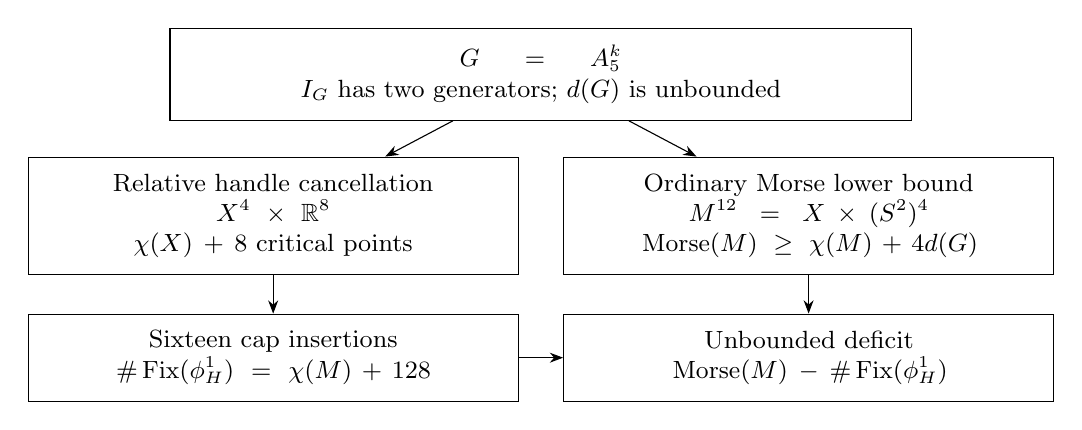
\begin{tikzpicture}[
 every node/.style={align=center,font=\small},
 box/.style={draw,inner sep=6pt,text width=58mm},
 >={Stealth}]
\node[box,text width=90mm] (group) at (0,0)
{$G=A_5^k$\\$I_G$ has two generators; $d(G)$ is unbounded};
\node[box] (morse) at (-3.4,-1.8)
 {Relative handle cancellation\\$X^4\times\R^8$\\$\chi(X)+8$ critical points};
\node[box] (bound) at (3.4,-1.8)
 {Ordinary Morse lower bound\\$M^{12}=X\times(S^2)^4$\\$\Morse(M)\ge\chi(M)+4d(G)$};
\node[box] (closed) at (-3.4,-3.6)
 {Sixteen cap insertions\\$\#\Fix(\phi_H^1)=\chi(M)+128$};
\node[box] (gap) at (3.4,-3.6)
 {Unbounded deficit\\$\Morse(M)-\#\Fix(\phi_H^1)$};
\draw[->] (group)--(morse);
\draw[->] (group)--(bound);
\draw[->] (morse)--(closed);
\draw[->] (bound)--(gap);
\draw[->] (closed)--(gap);
\end{tikzpicture}
\caption{The augmentation-ideal bound controls the constructed fixed-point
count. The group generator bound supplies the larger ordinary Morse
lower bound on the same closed manifold.}
\label{fig:construction}
\end{figure}

\subsection{Proof organization}
Section~\ref{sec:algebra} proves the two group-ring facts and the exact
row operation needed for geometric cancellation.
Section~\ref{sec:relative-model} constructs the relative Morse model and
its handle complex. Section~\ref{sec:cancellation} reduces the handle
counts while preserving the quadratic collars.
Section~\ref{sec:hamiltonian} realizes the local map on the closed product.
Section~\ref{sec:counting} compares the two counts and proves the theorem
and its deficit corollary.

\section{Group generators and augmentation ideals}
\label{sec:algebra}

We need finite groups whose group generators are numerous but whose
augmentation ideals have uniformly short generating lists.  The distinction
between these two numbers is classical; see
\cite[Sections~1--2]{GruenbergLinnell}.  We give the estimates needed here,
then prove the elementary row reduction used in the handle construction.
All modules in this section are right modules.

For a finitely generated group $G$, let $d(G)$ be its minimum number of
group generators.

\begin{lemma}\label{lem:group-gap}
Let $S$ be a nontrivial finite group, let $k$ be a finite positive
integer, and let $m\ge0$ be an integer.
If $k>|S|^m$, then $d(S^k)>m$.
\end{lemma}

\begin{proof}
Suppose that $g_1,\ldots,g_m$ generate $S^k$, padding a shorter list with
identities.  Each factor coordinate $i$ gives a tuple
$((g_1)_i,\ldots,(g_m)_i)\in S^m$.  Since $k>|S|^m$, two coordinates
$i\ne j$ have the same tuple.  Every listed generator then belongs to the
proper subgroup
\[
  \{g\in S^k:g_i=g_j\},
\]
a contradiction.
\end{proof}

We shall use
\begin{equation}\label{eq:group-choice}
  b=2,\qquad S=A_5,\qquad G=S^k.
\end{equation}
For now $k\ge1$ is arbitrary.  The group $S$ is nonabelian simple, hence
perfect, and the direct product $G$ is also perfect.  Every finite group is finitely presented: one may
take symbols $t_g$ for its elements and relations $t_1=1$ and
$t_gt_h=t_{gh}$.  Thus these groups satisfy the finite-presentation
condition needed for the symplectic realization below.

Write $\Lambda=\Z[G]$ and let
\[
  \operatorname{aug}:\Lambda\longrightarrow\Z,
  \qquad \sum_{g\in G}a_gg\longmapsto\sum_{g\in G}a_g
\]
be the augmentation map.  Its kernel $I$ is the augmentation ideal,
regarded as a right $\Lambda$-module.

The uniform bound below is a special case of the direct-product theorem
of Cossey, Gruenberg and Kov\'acs~\cite[Theorem~2]{CGK1974}.
For finite groups, that theorem expresses the augmentation-ideal
generator number of a direct product as the maximum of the corresponding
factor numbers and the generator number of its abelianization.
We give an elementary proof for the present family, including the
passage from modular to integral generators.

\begin{lemma}\label{lem:augmentation}
For every finite positive integer $k$, the right augmentation ideal of
$\Z[A_5^k]$ can be generated by two elements.
\end{lemma}

\begin{proof}
We first prove that two generators suffice modulo every prime.
The group $A_5$ is generated by
$a=(1\,2\,3\,4\,5)$ and $c=(1\,2\,3)$.
Indeed, $aca^{-1}=(2\,3\,4)$, and the subgroup generated by
$c$ and $aca^{-1}$ is transitive on $\{1,2,3,4\}$, and the
stabilizer of $4$ contains the order-three group generated by $c$. It is therefore all of the copy
of $A_4$ fixing $5$. The subgroup generated by $a,c$ is transitive
on five letters and has a stabilizer containing this $A_4$, so it
has order at least $5\cdot12=60$ and equals $A_5$.

Put $\Lambda=\Z[G]$ and $I=\ker(\aug:\Lambda\to\Z)$.
The splitting $\Lambda=I\oplus\Z\cdot1$ as abelian groups identifies
\[
 R_p=\F_p[G],\qquad I_p=I/pI=\ker(R_p\xrightarrow{\aug}\F_p).
\]
For each simple right $R_p$-module $V$, we claim
\begin{equation}\label{eq:augmentation-hom-bound}
 \dim_{\F_p}\Hom_{R_p}(I_p,V)\le 2\dim_{\F_p}V.
\end{equation}
If $G$ acts trivially on $V$, every homomorphism $\ell:I_p\to V$
defines a group homomorphism $g\mapsto\ell(g-1)$ to the additive
group of $V$. Since $G$ is perfect, this map vanishes, and thus
$\ell=0$.

Otherwise some factor $S_i\cong A_5$ acts nontrivially on $V$.
Normality of $S_i$ makes $V^{S_i}$ a submodule, so simplicity gives
$V^{S_i}=0$. Write $a_i,c_i$ for the two displayed generators in this
factor. We show that $\ell$ is determined by
$\ell(a_i-1)$ and $\ell(c_i-1)$. The identity
\[
 \ell(gh-1)=\ell(g-1)h+\ell(h-1)
\]
shows that if both values vanish, then $\ell(s-1)=0$ for every
$s\in S_i$. If $h$ lies in the product of the other factors, then
for every $s\in S_i$,
\[
 \ell(h-1)(s-1)
 =\ell((h-1)(s-1))
 =\ell((s-1)(h-1))=0.
\]
Thus $\ell(h-1)\in V^{S_i}=0$. Every element of $G$ has the form
$sh$, so the same identity gives $\ell=0$. Evaluation at the two
generators therefore embeds $\Hom_{R_p}(I_p,V)$ into $V^2$, proving
\eqref{eq:augmentation-hom-bound}.

Let $J=\Jac(R_p)$. We use the elementary finite-dimensional algebra
facts that $J$ annihilates every simple module, $J$ is nilpotent,
and $R_p/J$ is semisimple. For completeness, $J$ is the intersection
of the maximal right ideals, equivalently the annihilators of the
simple right modules. Multiplication by $J$ lowers a composition
series of the regular module, proving nilpotence. Finite dimension
allows finitely many maximal right ideals with intersection $J$;
thus $R_p/J$ embeds in a finite direct sum of simple quotients and is
semisimple, as are its finite-dimensional modules.

Let $a_V,t_V$ denote the multiplicities of a simple module $V$ in
$I_p/I_pJ$ and $R_p/J$, respectively, and let
$e_V=\dim_{\F_p}\End_{R_p}(V)$. Schur's lemma and evaluation at $1$
give
\[
 \dim_{\F_p}\Hom_{R_p}(I_p,V)=a_Ve_V,
 \qquad
 \dim_{\F_p}\Hom_{R_p}(R_p,V)=t_Ve_V=\dim_{\F_p}V.
\]
Consequently $a_V\le2t_V$ for every $V$. There is a surjection
$(R_p/J)^2\to I_p/I_pJ$. Lift the two generator images to $I_p$
and let $N_p$ be their right span. Then
$I_p/N_p=(I_p/N_p)J$, and nilpotence gives $N_p=I_p$.
Hence $I_p$ has a generating pair for every prime $p$.

It remains to lift to two integral generators. We first choose one
element whose right ideal has finite additive index in $I$, while
retaining a residue that extends to a generating pair at each prime
dividing $|G|$. A second element will then remove the finite quotient.
Put $n=|G|=60^k$.
For each $p\in\{2,3,5\}$ choose a generating pair
$(u_p,v_p)$ of $I_p$. By the Chinese remainder theorem on the free
abelian group $I$, choose $y_0\in I$ with residue $u_p$ at each of
these three primes. Define
\[
 z=n\cdot1-\sum_{g\in G}g\in I.
\]
For $x\in I$, we have $zx=nx$. Thus left multiplication on $I$ by
$y_0+30t z$ has matrix $L_{y_0}+30tn\,\mathrm{id}$. Its determinant
is a nonzero polynomial in $t$, so there is an integer $t$ for which
it is nonzero. Fix this $t$ and put
\[
 y_1=y_0+30t z,\qquad D=|\det(L_{y_1}:I\to I)|>0.
\]
The adjugate identity gives $DI\subset y_1I\subset y_1\Lambda$.
Moreover, $y_1$ still reduces to $u_p$ for $p=2,3,5$.

For each prime $p\mid D$, the right module $I_p/y_1R_p$ is cyclic.
For $p\mid n$, it is generated by the image of $v_p$.
For $p\nmid n$, the element
\[
 e_p=1-n^{-1}\sum_{g\in G}g\in R_p
\]
satisfies $I_p=e_pR_p$, so its image generates every quotient of
$I_p$, including $I_p/y_1R_p$. Apply the Chinese remainder theorem on $I$
to choose $y_2\in I$ reducing to $v_p$ when $p\mid D$ and $p\mid n$,
and to $e_p$ when $p\mid D$ and $p\nmid n$. When $D=1$,
take $y_2=0$.

The quotient $C=I/(y_1\Lambda+y_2\Lambda)$ is a finite abelian group
killed by $D$, and the residue choices give $C=pC$ for every prime
$p\mid D$. Iterating these equalities through the prime factorization
of $D$ yields $C=DC=0$. Therefore $y_1,y_2$ generate $I$ as a right
$\Lambda$-module.
\end{proof}

In particular, choosing any finite $k>60^{16b}$ gives
\begin{equation}\label{eq:generator-gap}
  d(G)>16b,
  \qquad I\text{ has a generating list of length }b.
\end{equation}
We always pad such a list by zeros if necessary.  Increasing $k$ makes
$d(G)$ unbounded by Lemma~\ref{lem:group-gap}, while
Lemma~\ref{lem:augmentation} keeps the same bound $b$.

\subsection{An elementary row reduction}

The next lemma supplies an entry equal to $1$ using only elementary
basis additions.  This is the form needed for handle slides.  It is a
special case of Bass's stable-range results applied to the opposite
ring~\cite[Lemma~6.4 and Theorems~4.2(a),~11.1]{Bass}; we include a direct
proof to retain control of the multiplication sides and the row length.

\begin{lemma}\label{lem:row}
Let $G$ be a finite group and $\Lambda=\Z[G]$.  If $m\ge3$ and
\[
  x_1\Lambda+\cdots+x_m\Lambda=\Lambda,
\]
then finitely many elementary additions
\[
  x_j\longleftarrow x_j+x_iq,
  \qquad i\ne j,\quad q\in\Lambda,
\]
can make an entry of the row equal to $1$.
\end{lemma}

\begin{proof}
We first record how to correct a designated entry over a
finite-dimensional semisimple algebra $R$.  Suppose $xR+U=R$, where
$U$ is a right ideal.  Let $T=L_x:R\to R$ be left multiplication by
$x$, let $\pi:R\to R/U$ be the quotient map, and put
$K=\ker(\pi T)$.  The map $\pi T$ is onto, and the split exact
sequences give
\[
  R\cong K\oplus R/U,
  \qquad R\cong U\oplus R/U.
\]
Comparison of simple-module multiplicities therefore gives $K\cong U$.
Choose an isomorphism $h:K\to U$.  Extend
$h-T|_K:K\to U$ to a right-module map $c:R\to U$ using a complement
of $K$.  The map $T+c$ is an isomorphism: it restricts to $h$ on $K$
and induces the isomorphism $R/K\to R/U$ supplied by $\pi T$.
Every right-module endomorphism of $R$ is left multiplication by its
value at $1$.  Hence $T+c=L_{x+u}$ for $u=c(1)\in U$, and $x+u$ is
a unit.  If $U=\sum_{i\ne j}x_iR$, this corrects only the designated
entry $x_j$ by additions of right multiples of the other entries.

Apply this observation first to $R=\Q[G]$, which is semisimple by
Maschke's theorem, with designated entry $x_1$.  In group-basis
coordinates for the correcting coefficients $q_i$, the determinant
\[
  \det_{\Q} L_{x_1+\sum_{i\ne1}x_iq_i}
\]
is a polynomial with integer coefficients.  The unit correction over
$\Q[G]$ shows that it is nonzero.  A nonzero polynomial over $\Q$
does not vanish at every integer tuple, by induction on its number of
variables.  We may therefore choose all $q_i\in\Lambda$ with this
determinant nonzero.  After these elementary additions, rename the
first entry $x_1$.  Its principal right ideal has finite additive index
\[
  D=[\Lambda:x_1\Lambda]=|\det L_{x_1}|,
  \qquad D\Lambda\subset x_1\Lambda.
\]

We keep this entry fixed and correct only $x_2$.  For each prime
$p\mid D$, let $R_p=\Lambda/p\Lambda$ and
$J_p=\operatorname{Jac}(R_p)$.  The current row generates the unit
right ideal in the semisimple algebra $R_p/J_p$.  The preceding
observation gives coefficients $\bar q_{i,p}\in R_p$, $i\ne2$, such
that
\[
  \bar x_2+\sum_{i\ne2}\bar x_i\bar q_{i,p}
\]
is a unit modulo $J_p$, and hence a unit in $R_p$.  Here units lift
across the nilpotent ideal $J_p$, since $1-j$ has a finite geometric
series inverse for $j\in J_p$.  Choose $q_i\in\Lambda$, $i\ne2$,
with these residues for all $p\mid D$ by coefficientwise Chinese
remaindering, and make the additions
\[
  x_2\longleftarrow x_2+\sum_{i\ne2}x_iq_i.
\]
All source entries remain fixed during these additions, so the new
$x_2$ is a unit modulo every prime dividing the unchanged integer $D$.

The additive quotient
$A=\Lambda/(x_1\Lambda+x_2\Lambda)$ is finite and killed by $D$.
For each $p\mid D$, the invertibility of $x_2$ modulo $p$ gives
$x_2\Lambda+p\Lambda=\Lambda$, and hence $A=pA$.  Iteration gives
$A=DA=0$.  This also covers $D=1$, when $A$ is already zero.
We have proved $x_1\Lambda+x_2\Lambda=\Lambda$.

Finally put $t=x_3$ and choose $a,c\in\Lambda$ with $x_1a+x_2c=1$.  The two
elementary additions to the third entry with coefficients
$a(1-t)$ and $c(1-t)$ give
\[
  t+x_1a(1-t)+x_2c(1-t)=1.
\]
Neither source entry changes, and all products retain the required
order.
\end{proof}

\section{A relative Morse model in twelve dimensions}
\label{sec:relative-model}

We now turn a short generating list for an augmentation ideal into a Morse
function with few critical points.  Let $G$ be a finite group, put
$\Lambda=\Z[G]$, and let $I\subset\Lambda$ be its right augmentation ideal.
Assume that $I$ has a generating list of length $b\geq2$.
We will use this list and the elementary-row lemma established above.
Let $X$ be a closed connected oriented smooth four-manifold with
$\pi_1(X)\cong G$.  Since $G$ is finite, rational homology and Poincar\'e
duality give
\[
 H_1(X;\Q)=H_3(X;\Q)=0,
 \qquad \chi(X)=2+\dim_{\Q}H_2(X;\Q)\geq 2.
\]
No symplectic structure is needed for this part of the argument.
The relation between quadratic stabilization, group-ring complexes and
augmentation generators is developed by Eliashberg and Gromov
\cite[Sections~0.2.2 and~0.2.5]{EliashbergGromov1998}.
We carry out the required realization on a specified relative cobordism,
so that the number of variables and the exterior function remain fixed.

For $u,v\in\R^4$, put
\begin{equation}
 Q(u,v)=\frac{|v|^2-|u|^2}{2},
 \qquad r^2=|u|^2+|v|^2.
 \label{eq:quadratic}
\end{equation}
We also write $Q$ for its pullback to $X\times\R^8$.

\begin{proposition}
\label{prop:relative-morse}
Let $G$ be a finite group whose right augmentation ideal in $\Z[G]$
has a generating list of length $b\geq2$.
Let $X$ be a closed connected oriented smooth four-manifold with
$\pi_1(X)\cong G$.
There is a smooth Morse function $F:X\times\R^8\to\R$ such that
\[
 F=Q\quad\text{for }r\geq 3,
 \qquad
 \#\Crit(F)=\chi(X)+4b.
\]
Its critical points have indices between four and eight.
\end{proposition}

The number of added variables is part of the assertion.  We will prove the
proposition by changing handles on one fixed compact twelve-dimensional
cobordism.  This section constructs the cobordism and its handle complex;
Section~\ref{sec:cancellation} performs the reduction and completes the proof.

\subsection{The domain and its collars}

Define
\begin{equation}
 \begin{gathered}
 E=\{(u,v):r^2\leq 9,\ -1\leq Q\leq 1\},
 \qquad E_{\pm}=E\cap\{Q=\pm1\},\\
 W=X\times E,\qquad A=X\times E_-,\qquad B=X\times E_+.
 \end{gathered}
 \label{eq:relative-domain}
\end{equation}
The incoming and outgoing faces are $A$ and $B$; the side is the face
$r=3$.  At its corners, both $u$ and $v$ are nonzero and $dr,dQ$ are
linearly independent.  In a neighborhood of the side, the coordinates
\[
 (r,Q,u/|u|,v/|v|)
\]
give a product collar with interval coordinate $Q$.  Since $dQ\neq0$ on
$A\cup B$, these faces also have collars with coordinate $Q$.  To make
the collars compatible, choose a vector field with $dQ$-value one which
is the product coordinate field near the side, and extend it over the
ends by a partition of unity.  All handle constructions below take place
away from a fixed smaller side collar.

Radial contraction preserves $E$, so $E$ is contractible.  On $E_-$,
the parametrization
\[
 (\xi,v)\longmapsto
 \bigl(\sqrt{2+|v|^2}\,\xi,v\bigr),
 \qquad \xi\in S^3,\quad |v|^2\leq\frac72,
\]
identifies $E_-$ with $S^3\times D^4$.  Interchanging $u$ and $v$ gives
the same description of $E_+$.  Consequently both inclusions
$A\hookrightarrow W$ and $B\hookrightarrow W$ induce isomorphisms on
fundamental groups.

Write $\widetilde X$ for the universal cover of $X$ and use tildes for
the corresponding covers of $W,A,B$.  The relative homology of
$(E,E_-)$ is $\Z$ in degree four and zero in every other degree.  The
relative K\"unneth formula therefore gives, equivariantly for the deck
action,
\begin{equation}
 H_{4+i}(\widetilde W,\widetilde A;\Z)
 \cong H_i(\widetilde X;\Z).
 \label{eq:relative-homology}
\end{equation}
There is no torsion term because the relative homology of $(E,E_-)$ is
free.  The same formula holds with $\widetilde B$ in place of
$\widetilde A$.  In particular,
\begin{equation}
 H_4(\widetilde W,\widetilde A;\Z)\cong\Z,
 \qquad H_5(\widetilde W,\widetilde A;\Z)=0,
 \label{eq:low-relative-homology}
\end{equation}
where the action on $\Z$ is trivial.  Here we used connectedness and
simple connectedness of $\widetilde X$.

\subsection{An initial height function}

Choose a Morse function $f:X\to\R$ with one minimum and one maximum.
For completeness, this follows from the usual handle description of a
connected manifold.  After ordering the handles, the zero- and
one-handles form a connected graph.  Cancelling the edges of a spanning
tree against all but one zero-handle leaves one minimum.  Attachments
above each cancelling pair are transferred through the resulting
boundary identification.  Applying the same procedure to the dual
handle decomposition removes the extra maxima without changing the
minimum.  This uses the handle decomposition theorem and the geometric
cancellation criterion, in their elementary zero/one-handle cases
\cite[Theorem~2.22 and Lemma~8.24]{Ranicki2002}.

Let $\eta:[0,\infty)\to[0,1]$ be smooth, equal to one near zero and
supported in $[0,1)$.  For $\sigma>0$ sufficiently small, set
\begin{equation}
 h_0(x,u,v)=Q(u,v)+\sigma\eta(r^2)f(x).
 \label{eq:initial-height}
\end{equation}
Choose $\sigma$ so that
\[
 \sigma\|f\|_{\infty}<\frac12,
 \qquad
 2\sigma\|f\|_{\infty}\|\eta'\|_{\infty}<1.
\]
The perturbation is supported where $r<1$ and hence $|Q|<1/2$.
Thus $h_0(W)\subset[-1,1]$, and $h_0=Q$ near every face of $W$.
For $r>0$, its derivative in the extra variables has norm at least
\[
 r\bigl(1-2\sigma\|f\|_{\infty}\|\eta'\|_{\infty}\bigr)>0.
\]
At $r=0$, the critical-point equation is $df=0$, and the Hessian is
the direct sum of $\sigma\operatorname{Hess}f$ and
$\operatorname{Hess}Q$.  Therefore $h_0$ is Morse, with exactly the
critical points of $f$, each shifted upward by four in index.  In
particular it has one critical point of index four and one of index
eight.

\subsection{Levels and the relative handle complex}

Use gradient-like fields which are product fields on the side collar.
The Morse--handle correspondence then describes $(W;A,B)$ by handles
attached in the interiors of its regular levels.  The standard local
handle traces and their product regions give this correspondence
relative to the side collar; see
\cite[Proposition~2.20 and Theorem~2.22]{Ranicki2002} for the handle
construction.  Only handles of indices $4,\ldots,8$ will occur.

We may order these handles by index.  Indeed, if an index-$j$ handle
is followed by an index-$\ell$ handle with $\ell\leq j$, the latter
attaching sphere has dimension $\ell-1$, and the former belt sphere
has dimension $11-j$ in the intervening eleven-dimensional level.
Their dimension sum is
\[
 (\ell-1)+(11-j)=10+\ell-j<11.
\]
General position makes the attaching sphere disjoint from that belt
sphere.  After shrinking its framed neighborhood, it can be moved
back through the surgery, interchanging the two handles.  All later
attachments are transferred through the induced identification of
the upper level.  The same argument permits arbitrary ordering
within an equal-index block, with all moves supported in the interior.

Every regular level $L$ is connected, and its inclusion into $W$
induces
\begin{equation}
 \pi_1(L)\cong\pi_1(W)\cong G.
 \label{eq:level-fundamental-group}
\end{equation}
To see this directly, surgery for an index-$j$ handle removes a
neighborhood of $S^{j-1}$ and inserts one of $S^{11-j}$.  For
$4\leq j\leq8$, both spheres have dimension at least three and
codimension at least four in the level.  General position and van
Kampen show that these surgeries preserve connectedness and the
fundamental group.  Start with $A$, whose inclusion into $W$ is a
fundamental-group isomorphism.  Alternatively, from any intermediate
level both the upper part and the reversed lower part are built with
handles of index at least four, so neither part changes the
fundamental group.  The interior of $L$ has the same fundamental
group as $L$.

Choose an orientation and a lift of each handle.  Regard the deck
action as a right action: if it was originally written on the left
as $D_g$, use $c\cdot g=D_{g^{-1}}c$.  Let $C_i$ be the based free
right $\Lambda$-module generated by the handles of index $4+i$, and
let $r_i$ be their number.  The resulting relative handle complex is
\begin{equation}
 0\longrightarrow C_4\xrightarrow{\partial_4}C_3
 \xrightarrow{\partial_3}C_2\xrightarrow{\partial_2}C_1
 \xrightarrow{\partial_1}C_0\longrightarrow0,
 \qquad C_i\cong\Lambda^{r_i}.
 \label{eq:handle-complex}
\end{equation}
Its degree-$i$ homology is
$H_{4+i}(\widetilde W,\widetilde A;\Z)$.  One way to obtain the
complex is to filter the handle decomposition by index; each
successive relative group is freely generated by the lifted handles
in that index.  Boundary coefficients are signed intersections of
lifted attaching spheres with lifted belt spheres one index lower.
Thus, writing
\[
 \partial e_j=\sum_i e_i a_{ij},
\]
the entries $a_{ij}$ lie in $\Lambda$ and multiply the basis elements
on the right.  Replacing a basis vector $e_j$ by $e_j+e_i q$, with $i\neq j$, adds
column$_i\,q$ to column$_j$ in its outgoing differential.  If $T$
is the elementary matrix of this basis change, the adjacent
differentials change coherently as $D\mapsto DT$ and
$D'\mapsto T^{-1}D'$.  These conventions will be used for the handle
slides in Section~\ref{sec:cancellation}.

\begin{lemma}
\label{lem:handle-complex}
For any relative handle presentation of this same $(W;A,B)$ with
indices in $4,\ldots,8$ and $r_0=r_4=1$, its based right-module
complex satisfies
\begin{equation}
 \operatorname{im}\partial_1=I,
 \qquad
 \operatorname{im}\partial_2=\ker\partial_1,
 \qquad
 r_2=\chi(X)-2+r_1+r_3\geq r_1,
 \label{eq:handle-identities}
\end{equation}
where $C_0$ is identified with $\Lambda$ using its chosen basis.
The same assertions hold for the reversed cobordism relative to $B$.
\end{lemma}

\begin{proof}
By \eqref{eq:low-relative-homology}, the quotient
$C_0/\operatorname{im}\partial_1$ is the trivial right module $\Z$.
A surjective right-module map $\Lambda\to\Z$ sends $1$ to $1$ or
$-1$, so its kernel is $I$.  The vanishing of relative homology in
degree five gives the second equality.

Since $E$ is contractible and $E_-$ has the homotopy type of $S^3$,
we have $\chi(W,A)=\chi(X)$.  All handle indices have been shifted
by the even number four, and hence
\[
 \chi(X)=r_0-r_1+r_2-r_3+r_4
         =2-r_1+r_2-r_3.
\]
This gives the rank identity; its inequality follows from
$\chi(X)\geq2$ and $r_3\geq0$.  Finally, the same relative covering
homology computation holds with $B$ in place of $A$.  Reversal sends
index $4+i$ to index $8-i$ and preserves the endpoint counts, so the
argument applies unchanged.
\end{proof}

We have now constructed a height on the required fixed cobordism
and identified the algebra that its handles must satisfy.  To finish
Proposition~\ref{prop:relative-morse}, it remains to reduce the
index-five and index-seven counts to $b$ while retaining the single
index-four and index-eight handles and the prescribed collars.
Then Lemma~\ref{lem:handle-complex} will force
$r_2=\chi(X)-2+2b$ and the total count $\chi(X)+4b$.

\section{Geometric reduction of the handles}
\label{sec:cancellation}

We continue with the fixed cobordism $(W;A,B)$ and the conventions of
Section~\ref{sec:relative-model}.  The aim is to retain just $b$ handles
in each of indices five and seven.  There are two distinct steps:
elementary operations produce a coefficient exactly equal to $1$, and
Whitney moves turn that coefficient into one geometric intersection.
All moves below occur in the interior of $W$.

\subsection{Introducing the augmentation generators}

A slide of one index-$j$ handle over another replaces a basis vector
$e_j$ by $e_j+e_iq$ in the associated free right $\Lambda$-module.
To realize this, first take $q=\pm g$, with $g\in G$: choose a band
whose path represents $g$, and choose its orientation to give the sign.
The slide arcs can be chosen embedded and disjoint from the other
attaching cores in an eleven-dimensional level; their tubular
neighborhoods can then be shrunk as needed.  Repeated slides
realize an arbitrary finite integral combination of group elements.
The framing is carried through the band construction.  This is the
usual labelled handle slide; see \cite[proof of Theorem~4.2,
pp.~9--10]{Morgan2020}.  The two adjacent differentials change together
as described in Section~\ref{sec:relative-model}.

Write $e_1,\ldots,e_s$ for the existing index-five handles and
$a_i=\partial_1e_i\in I$.  By Lemma~\ref{lem:handle-complex}, the $a_i$
generate $I$ as a right ideal.  Fix a generating list
$y_1,\ldots,y_b$ for $I$, padded with zeros if necessary.

Introduce $b$ cancelling pairs of indices five and six, with new lower
handles $n_1,\ldots,n_b$ satisfying $\partial_1n_j=0$.
Here is a relative placement of the births.  In the level just after
the index-four handle, choose disjoint small balls missing its belt
sphere and all old index-five attaching cores.  These cores and the
belt sphere have dimensions four and seven, respectively, so their
finite union has empty interior.  After choosing the balls, shrink the
old attaching neighborhoods to miss them.  The balls then survive the
old index-five attachments.  Their product traces support ordinary
local five/six births.  When ordering the resulting handles by index,
pull the new lower attaching spheres back along these product traces.
They still miss the index-four belt sphere, so their boundary columns
are zero as asserted.

Choose coefficients in $\Lambda$ such that
\[
 y_j=\sum_{i=1}^s a_iq_{ij},
 \qquad
 a_i=\sum_{j=1}^b y_jt_{ji}.
\]
First slide each new handle to replace $n_j$ by
$n_j+\sum_i e_iq_{ij}$.  Its new column is $y_j$.
Next replace each old handle by $e_i-\sum_j n_jt_{ji}$, using the
new bases.  Every old column is now zero.  The new $b$ columns still
generate $I$.

\subsection{Producing a cancellable pair}

\noindent\emph{A coefficient equal to one.}
Select an old index-five handle $e$, and place it last among the
index-five handles.  Since $\partial_1e=0$, exactness in
Lemma~\ref{lem:handle-complex} gives $e\in\operatorname{im}\partial_2$.
If $h_1,\ldots,h_m$ are the index-six handles and $x_j$ is the
$e$-coefficient in $\partial_2h_j$, it follows that
\[
 x_1\Lambda+\cdots+x_m\Lambda=\Lambda.
\]
While an old handle remains, $r_1\geq b+1$; hence
$m=r_2\geq r_1\geq b+1\geq3$ by \eqref{eq:handle-identities}.
Lemma~\ref{lem:row} therefore applies.  Slides among the index-six
handles produce one whose coefficient into $e$ is exactly $1$.
Place this handle first among the index-six handles, immediately
after $e$.

\smallskip
\noindent\emph{Removing the extra intersections.}
Let $L$ be the intervening regular level, $T\cong S^5$ the upper
handle's attaching core sphere, and $D\cong S^6$ the lower handle's
belt sphere.  Their signed, group-labelled intersection is $1$.
For each group label, pair intersection points with opposite signs,
leaving exactly one positive point with identity label.  This pairing
is possible because all nonidentity coefficients vanish and the
identity coefficient is one.  In particular, the argument uses the
specific coefficient $1$, rather than an arbitrary unit of $\Lambda$.

For each pair, choose arcs joining its points on $T$ and on $D$.
The two spheres are simply connected.  Equality of the group labels
means that the resulting Whitney loop is null-homotopic in $W$.
By \eqref{eq:level-fundamental-group}, it is null-homotopic in $L$.
It therefore bounds a disk in the interior of $L$.  General position
makes this disk embedded, with interior disjoint from $T$, $D$,
the other disks, and the other attaching or belt cores that must be
retained.  The relevant inequalities are
\[
 2+5<11,\qquad 2+6<11,\qquad 2+2<11,
 \qquad 2+7<11.
\]
The last inequality covers the largest other core that occurs in
our index range.  Boundary arcs can likewise be chosen to miss the
other cores and intersection points.  All of these are finite,
compact constructions in $\operatorname{int}L$.

The high-dimensional Whitney theorem now removes each paired
intersection by an isotopy of $T$.  Its hypotheses are complementary
sphere dimensions at least three, opposite intersection signs, and
the null-homotopic Whitney loop just established; simple connectedness
of $L$ is not required.  The framing step is part of this theorem:
the normal splitting along the boundary of the Whitney disk extends
across it.  In the present dimensions the frame-extension space is
$V_4(\R^9)=O(9)/O(5)$, which is simply connected.
See \cite[Theorem~6.6 and Lemma~6.13]{Milnor1965}, or the group-ring
formulation in \cite[Theorem~7.27(i) and Corollary~7.30]{Ranicki2002}.
Transport the existing normal framing of $T$ through its isotopy.
We do not require that this entire handle framing extend over the
Whitney disk.

For support, first arrange the Whitney disks and their compact move
neighborhoods to miss the other cores; then shrink the other tubular
attaching neighborhoods to miss those supports.  A dimension argument
alone would not give disjointness from preassigned full-dimensional
neighborhoods.  The selected belt sphere remains the reference sphere
against which intersections are counted; the isotopy of the attaching
sphere removes intersections with it.  After the finite sequence of
Whitney moves, $T$ meets $D$ transversely in exactly one point.

\smallskip
\noindent\emph{Cancellation relative to the boundary.}
The geometric handle cancellation criterion now applies
\cite[Lemma~8.24]{Ranicki2002}.  We spell out its relative support
here because the quadratic collars must survive.  Isolate the two
adjacent critical points in a slab containing no others, and use a
descending gradient-like field that is a product on the side collar.
The single transverse intersection gives precisely one connecting
trajectory from the index-six point to the index-five point.  Choose
a regular level $c$ between the slab's bottom and the lower critical
value.  Every other nonconstant trajectory in the upper point's unstable manifold
crosses $c$.  Indeed, a trajectory that remained above $c$ could not
escape through the product side; compactness and strict decrease of
the height would force convergence to the only lower critical point,
contrary to uniqueness of the connecting trajectory.

A product side collar has an invariant inner boundary, which the
unstable manifold cannot cross.  Retain a strictly smaller side collar
outside that boundary.  The closure of the unstable manifold above
$c$ then lies in the compact part of the slab between $c$ and the
upper critical value, away from the retained collar and the slab's ends.
This closure can include limiting trajectories through the lower
critical point; it need not be a smooth disk.
The local Morse cancellation theorem gives a deformation supported
in any sufficiently small neighborhood of this closure, fixed elsewhere
\cite[Theorem and Corollary~1]{Laudenbach2013}.
One can apply its closed-manifold formulation by first extending the
height and field to a closed enlargement; they agree on the slab,
and the deformation restricts to the same $W$.
Thus the cancellation changes neither the earlier handles nor the
side and end collars.  The upper attaching maps are transferred
through the induced identification of levels.

For clarity, the chosen index-six column may also have coefficients
into other lower handles.  In bases beginning with the selected pair,
its differential has the block form
\[
 \partial_2=
 \begin{pmatrix}1&a\\ v&B\end{pmatrix},
 \qquad \partial_1=(0\ \ d),\qquad dv=0.
\]
Cancellation leaves $B-va$ as the next differential and leaves $d$
unchanged.  This records algebraically why one coefficient equal to
one suffices and why the other old zero columns of $\partial_1$
survive.  Geometrically this is the preservation of the lower handles
and transfer of the upper attachments just described.

\smallskip
\noindent\emph{Iteration.}
We can therefore repeat the construction until every old index-five
handle has been removed.  Each step cancels one handle of index five
and one of index six.  The identities of Lemma~\ref{lem:handle-complex}
continue to hold for the same cobordism, and the $b$ new lower handles
remain.  At the end,
\[
 r_1=b.
\]

\subsection{The reverse reduction and the quadratic collars}

Turn the cobordism around.  Near its faces the new height is $-Q$,
and an original handle of index $4+i$ has reversed index $8-i$.
The relative covering homology for $(W,B)$ is the same as for $(W,A)$,
so the preceding construction applies without changing the dimension
or adding any variables.  It reduces the reversed index-five count
to $b$, that is, the original index-seven count to $b$.
Reversed five/six births and cancellations are original seven/six
births and cancellations.  They preserve the number $r_1=b$ of original
index-five handles; the upper attaching data in the reversed
presentation are transferred as needed.  Both endpoint counts remain
one.  Lemma~\ref{lem:handle-complex} now gives
\begin{equation}
 (r_0,r_1,r_2,r_3,r_4)
   =\bigl(1,b,\chi(X)-2+2b,b,1\bigr).
 \label{eq:final-handle-counts}
\end{equation}

The handle traces and their intervening product regions supply an
actual smooth Morse height on the same $W$.  Since only finitely many
compactly supported moves were used, a common smaller side collar
still has height $Q$.  We may also prescribe height $-1$ and $1$ on
the two end faces and make its inward derivative strictly positive
at the incoming end and strictly negative at the outgoing end.
It remains to ensure equality with $Q$ on whole end collars, compatible
with the side collar.

At $A$, use the inward coordinate $s=Q+1$.  On a sufficiently small
collar the height has the form
\[
 -1+s\,a(y,s),\qquad a(y,s)>0,
\]
and $a=1$ near the side.  Replace it by
\[
 -1+s\bigl[1+\theta(s)(a(y,s)-1)\bigr],
\]
where $0\leq\theta\leq1$, with $\theta=0$ close to $s=0$ and
$\theta=1$ farther inside.
Put $c_0=\min(1,\inf a)>0$.  Its normal derivative is
\[
 1+\theta(a-1)+s\theta\,\partial_sa+s\theta'(a-1).
\]
The first two terms together are at least $c_0$.  Choose the collar
so small that $|s\partial_sa|<c_0/4$, and choose the transition so
slowly in $\log s$ that
$|s\theta'|\,\|a-1\|_\infty<c_0/4$.
For example, a fixed smooth transition applied to
$\log(s/s_0)/L$, with $L$ large and then $s_0$ sufficiently small,
has these properties and is constant near both endpoints.
The normal derivative is then at least $c_0/2$.
This introduces no critical points and leaves the side collar fixed.
Apply the identical argument at $B$ to one minus the height with
inward coordinate $1-Q$.

The final height equals $Q$ near every face and corner of $W$.
Extend it by $Q$ to $X\times\R^8$ and call the result $F$.
This extension is smooth across all seams.  Its exterior has no
critical points because $dQ=0$ only on the zero section, which lies
in the interior of $W$.  It equals $Q$ for $r\geq3$ and, by
\eqref{eq:final-handle-counts}, has exactly
\[
 1+b+\bigl(\chi(X)-2+2b\bigr)+b+1=\chi(X)+4b
\]
critical points.  This completes the proof of
Proposition~\ref{prop:relative-morse}.

\section{Closing the Hamiltonian model}
\label{sec:hamiltonian}

We now turn a Morse function with eight quadratic variables into a
Hamiltonian map on a closed manifold.  Each of the sixteen products of
north and south sphere caps will contain one copy of its critical set.
The rotations outside the caps must be chosen with care: their endpoint
maps agree with the quadratic model at both poles, although their paths
can differ by full turns. We track this difference to identify the
homotopy classes of the resulting fixed-point loops as well.

\begin{proposition}\label{prop:cap-transfer}
Let $(X,\omega_X)$ be a closed connected symplectic four-manifold. Write
$(u,v)\in\R^4\times\R^4$ and set
\[
 Q(u,v)=\frac{|v|^2-|u|^2}{2},
 \qquad r^2=|u|^2+|v|^2.
\]
Suppose that $F\colon X\times\R^8\to\R$ is a smooth Morse function
such that $F=Q$ whenever $r\ge3$, and let $N=\#\Crit(F)$.
Let $\sigma$ be the standard area form of total area $4\pi$ on the unit
sphere. For every $\lambda>25/2$, the closed symplectic manifold
\[
 (M,\omega_M)=
 \left(X\times(S^2)^4,
 \omega_X+\lambda\sum_{j=1}^4\sigma_j\right)
\]
admits a Hamiltonian $H\in C^\infty((\R/\mathbb Z)\times M,\R)$ such
that every fixed point of $\phi_H^1$ is nondegenerate, every loop
$t\mapsto\phi_H^t(p)$ based at a fixed point $p$ is contractible in
$M$, and
\[
 \#\Fix_0(\phi_H^1;H)=\#\Fix(\phi_H^1)=16N.
\]
Here $\sigma_j$ denotes the pullback of $\sigma$ from the $j$th sphere,
and Hamiltonian vector fields satisfy $\omega_M(X_H,\cdot)=dH$.
\end{proposition}

We first record the local short-period estimate used below. Yorke proved
the sharp lower bound $2\pi/L$ for a nonconstant periodic solution of a
Euclidean vector field with Lipschitz constant $L$~\cite{Yorke1969}.
The weaker coordinate estimate here suffices on a compact invariant set.

\begin{lemma}\label{lem:short-period}
Let $V$ be a smooth vector field on a smooth manifold, with flow
$\Phi^t$, and let $K$ be a compact set on which this flow is defined
for all times and which it preserves. There is a number $\tau_0>0$
such that, for $p\in K$ and $0<\tau<\tau_0$,
\[
 \Phi^\tau(p)=p\quad\Longleftrightarrow\quad V(p)=0.
\]
\end{lemma}

\begin{proof}
Choose finitely many charts with image the Euclidean ball of radius
$3$, whose inverse images of the unit ball cover $K$. Let $C\ge1$
bound both the coordinate vector fields and their first derivatives
on the closed balls of radius $2$, and put $\tau_0=1/(2C)$.
If $0<\tau<\tau_0$, a trajectory
$t\mapsto\Phi^{\tau t}(p)$, $0\le t\le1$, with $p\in K$ stays
in the radius-$2$ ball of a chart whose unit ball contains $p$:
a first exit would require coordinate displacement greater than $1$,
whereas the speed bound gives displacement at most $\tau C<1/2$.
If the trajectory is a loop, write $w$ for its coordinate expression
and $\widehat V$ for the coordinate vector field. Then
\[
 \dot w(t)=\tau\widehat V(w(t)),\qquad
 \int_0^1\widehat V(w(t))\,dt=0.
\]
Set $S=\max_t|\widehat V(w(t))|$. Since
$|w(t)-w(a)|\le\tau S$ for $a,t\in[0,1]$, subtracting the zero
average and using the Lipschitz bound on this convex ball gives
\[
 |\widehat V(w(t))|
 \le\int_0^1|\widehat V(w(t))-\widehat V(w(a))|\,da
 \le C\tau S.
\]
Thus $S=0$, so the loop is constant and $V(p)=0$. The converse follows
from uniqueness of solutions. No homotopy assumption on the loop is used.
\end{proof}

\begin{proof}[Proof of Proposition~\ref{prop:cap-transfer}]
\emph{The local flows.}
Identify $\R^8$ with $\C^4$ by writing
\[
 u=(x_1,y_1,x_2,y_2),\qquad
 v=(x_3,y_3,x_4,y_4),\qquad z_j=x_j+iy_j,
\]
and equip $X\times\C^4$ with
$\Omega=\omega_X+\sum_jdx_j\wedge dy_j$.
Put $s_1=s_2=-1$ and $s_3=s_4=1$, so that
$Q=\frac12\sum_js_j|z_j|^2$.
Let $\Phi_F^\tau$ and $\Phi_Q^\tau$ denote the autonomous Hamiltonian
flows for this form and the stated sign convention.  In a standard
plane, $X_H=(H_y,-H_x)$; consequently
\begin{equation}\label{eq:quadratic-rotation}
 \Phi_Q^\tau(x,z_1,\ldots,z_4)
 =\bigl(x,e^{-is_1\tau}z_1,\ldots,e^{-is_4\tau}z_4\bigr).
\end{equation}

The vector fields of $F$ and $Q$ agree on $r\ge3$, including its
boundary.  That boundary is invariant, so uniqueness of solutions in
both time directions makes $r<3$ invariant as well.  Trajectories there
remain in the compact set $X\times\{r\le3\}$, whereas exterior
trajectories are the explicit rotations in
\eqref{eq:quadratic-rotation}.  Thus both flows are complete.  They
preserve the open set
\[
 U_0=X\times\{z\in\C^4:|z_j|<4\text{ for all }j\}
\]
and its compact closure $K$: points with $r<3$ have every $|z_j|<3$,
and exterior trajectories preserve each $|z_j|$.
Since $dQ\ne0$ on $r\ge3$, all critical points of $F$ lie in $r<3$.
They form a closed discrete subset of $X\times\{r\le3\}$ and hence
are finite.

\smallskip
\noindent\emph{One small time for all fixed points.}
We choose $\epsilon>0$ so that the fixed points of
$\Phi_F^\epsilon$ in $K$ are precisely the critical points of $F$,
all nondegenerate. Lemma~\ref{lem:short-period}, applied to $X_F$ on
the compact invariant set $K$, supplies $\tau_0>0$ for the first
assertion. The zero set of $X_F$ equals $\Crit(F)$ because $\Omega$
is nondegenerate. We next choose the time small enough to obtain
nondegeneracy of the return map as well.

At a critical point $p$, put $A_p=D_pX_F$.  Differentiating
$\Omega(X_F,\cdot)=dF$ at $p$, where $X_F(p)=0$, shows that $A_p$
is the composition of the nonsingular Hessian of $F$ with a symplectic
identification, and is therefore invertible.  Moreover,
\[
 D_p\Phi_F^\epsilon=\exp(\epsilon A_p).
\]
Let $R\ge1$ bound the moduli of all complex eigenvalues of the finitely
many matrices $A_p$.  If $0<\epsilon R<2\pi$, no nonzero eigenvalue
$\mu$ of any $A_p$ satisfies $\epsilon\mu\in2\pi i\mathbb Z$.
The eigenvalues of $\exp(\epsilon A_p)$ therefore all differ from one.
Fix, once and for all,
\begin{equation}\label{eq:small-epsilon}
 0<\epsilon<\min\{\pi,\tau_0,2\pi/R\}.
\end{equation}
This proves the required fixed-point and nondegeneracy assertions for
the local time-$\epsilon$ map.

\smallskip
\noindent\emph{Sphere caps and matching rotations.}
On each sphere use polar coordinates $(\vartheta,\varphi)$ and write
$h=\cos\vartheta$.  Its symplectic form is
\[
 \lambda\sigma
 =\lambda\sin\vartheta\,d\vartheta\wedge d\varphi
 =-\lambda\,dh\wedge d\varphi.
\]
The north and south cap coordinates are, respectively,
\begin{equation}\label{eq:pole-coordinates}
 z_N=\sqrt{2\lambda(1-h)}\,e^{i\varphi},
 \qquad
 z_S=\sqrt{2\lambda(1+h)}\,e^{-i\varphi}.
\end{equation}
These are smooth coordinates at their poles.  Indeed, in the usual
embedding coordinates $(a,b,h)$ of the unit sphere, they are
\[
 z_N=\sqrt{\frac{2\lambda}{1+h}}(a+ib),
 \qquad
 z_S=\sqrt{\frac{2\lambda}{1-h}}(a-ib).
\]
To check the area forms, write $z=R_ze^{i\psi}$.  At the north pole
$R_zdR_z=-\lambda dh$ and $d\psi=d\varphi$; at the south pole
$R_zdR_z=\lambda dh$ and $d\psi=-d\varphi$.  In both cases
$dx\wedge dy=R_zdR_z\wedge d\psi=-\lambda dh\wedge d\varphi$.

The two radius-$5$ caps are disjoint because $\lambda>25/2$:
their height intervals are
\[
 h>1-\frac{25}{2\lambda}
 \quad\text{and}\quad
 h<-1+\frac{25}{2\lambda}.
\]
For each choice $\nu\in\{N,S\}^4$, let $U_\nu\subset M$ be the
product of $X$ with the corresponding four radius-$4$ caps, and let
$\iota_\nu\colon U_0\to U_\nu$ be the symplectic identification
given by \eqref{eq:pole-coordinates}.  The sixteen sets $U_\nu$ are
pairwise disjoint.

For each $j$ choose a smooth function
$\alpha_j\colon[-1,1]\to(0,2\pi)$, constant on the radius-$5$ caps,
with the following values:
\[
\begin{array}{c|cc}
 &\text{north}&\text{south}\\ \hline
 s_j=-1&\epsilon&2\pi-\epsilon\\
 s_j=1&2\pi-\epsilon&\epsilon
\end{array}
\]
Smooth interpolation is possible within
$[\epsilon,2\pi-\epsilon]\subset(0,2\pi)$.
Define the Hamiltonian on $M$
\[
 P=\sum_{j=1}^4P_j(h_j),\qquad
 P_j(h)=\lambda\int_0^h\alpha_j(\xi)\,d\xi,
\]
and denote its flow by $\Psi_t$.  Since
\[
 \iota_{\alpha_j(h)\partial_\varphi}
       (-\lambda\,dh\wedge d\varphi)
 =\lambda\alpha_j(h)\,dh=dP_j,
\]
this flow rotates $\varphi_j$ with positive speed $\alpha_j(h_j)$
and fixes the $X$ coordinate.  A north coordinate rotates by
$e^{i\alpha_jt}$ and a south coordinate by $e^{-i\alpha_jt}$.
The table therefore gives the endpoint multiplier $e^{-is_j\epsilon}$
in either chart, and hence
\begin{equation}\label{eq:cap-endpoint-match}
 \iota_\nu^{-1}\circ\Psi_1\circ\iota_\nu=\Phi_Q^\epsilon
 \quad\text{on }U_0.
\end{equation}
Only the endpoints are equal: for some cap choices the rotation paths
differ by a full turn. Figure~\ref{fig:pole-rotations} illustrates this
distinction in one complex coordinate.

\begin{figure}[ht]
\centering
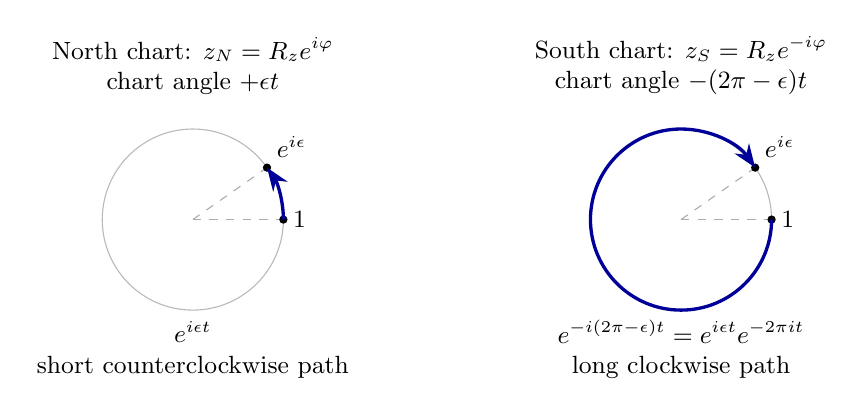
\begin{tikzpicture}[>=Stealth,every node/.style={font=\small},
                    x=1cm,y=1cm]
\begin{scope}[xshift=-3.1cm]
 \node[align=center] at (0,1.95)
   {North chart: $z_N=R_z e^{i\varphi}$\\
    chart angle $+\epsilon t$};
 \draw[gray!55] (0,0) circle (1.15);
 \draw[gray!65,dashed] (0,0)--(1.15,0);
 \draw[gray!65,dashed] (0,0)--(35:1.15);
 \fill (1.15,0) circle (1.5pt);
 \fill (35:1.15) circle (1.5pt);
 \node[right] at (1.15,0) {$1$};
 \node[above right] at (35:1.15) {$e^{i\epsilon}$};
 \draw[blue!60!black,very thick,->]
   (1.15,0) arc[start angle=0,end angle=35,radius=1.15];
 \node[align=center] at (0,-1.65)
   {$e^{i\epsilon t}$\\short counterclockwise path};
\end{scope}
\begin{scope}[xshift=3.1cm]
 \node[align=center] at (0,1.95)
   {South chart: $z_S=R_z e^{-i\varphi}$\\
    chart angle $-(2\pi-\epsilon)t$};
 \draw[gray!55] (0,0) circle (1.15);
 \draw[gray!65,dashed] (0,0)--(1.15,0);
 \draw[gray!65,dashed] (0,0)--(35:1.15);
 \fill (1.15,0) circle (1.5pt);
 \fill (35:1.15) circle (1.5pt);
 \node[right] at (1.15,0) {$1$};
 \node[above right] at (35:1.15) {$e^{i\epsilon}$};
 \draw[blue!60!black,very thick,->]
   (1.15,0) arc[start angle=0,end angle=-325,radius=1.15];
 \node[align=center] at (0,-1.65)
   {$e^{-i(2\pi-\epsilon)t}=e^{i\epsilon t}e^{-2\pi it}$\\
    long clockwise path};
\end{scope}
\end{tikzpicture}
\caption{The case $s_j=-1$, shown as multiplier paths in the two local
complex charts with angles drawn schematically. Both sphere longitudes increase,
but the south chart reverses their angular orientation. The paths
start at $1$ and end at the same multiplier $e^{i\epsilon}$; the
south path makes one additional negative turn. For $s_j=1$, the
north path makes the additional turn and both endpoints are
$e^{-i\epsilon}$.}
\label{fig:pole-rotations}
\end{figure}

Every $\Psi_t$ preserves all cap radii, so it preserves each $U_\nu$
and the complement of their union.  A nonpolar sphere point cannot be
fixed by $\Psi_1$, because its rotation angle lies strictly between
zero and $2\pi$.  Consequently
\begin{equation}\label{eq:rotation-fixed-set}
 \Fix(\Psi_1)=X\times\{N,S\}^4
 \subset\bigcup_\nu U_\nu.
\end{equation}

\smallskip
\noindent\emph{A correction supported inside the caps.}
We use the elementary composition rule that if Hamiltonian paths
$a_t,b_t$ have generators $A_t,B_t$, then $a_t\circ b_t$ has generator
$A_t+B_t\circ a_t^{-1}$.  Its vector field is
$X_{A_t}+(a_t)_*X_{B_t}$, and symplectic transport gives
$(a_t)_*X_{B_t}=X_{B_t\circ a_t^{-1}}$, proving the rule with our
sign convention.

On the model space define
\begin{equation}\label{eq:local-correction}
 \delta_t=\Phi_F^{\epsilon t}\circ\Phi_Q^{-\epsilon t},
 \qquad
 K_t=\epsilon\bigl(F-Q\circ\Phi_F^{-\epsilon t}\bigr),
 \qquad 0\le t\le1.
\end{equation}
The composition rule shows that $K_t$ generates $\delta_t$.
When $r\ge3$, the backward $F$ flow equals the backward $Q$ flow and
preserves $Q$.  Thus $K_t=0$ and $\delta_t=\operatorname{id}$ there.
Both constituent flows preserve $r<3$, so $\delta_t$ preserves $U_0$.
Uniformly in $t$, the support of $K_t$ is contained in the compact
set $X\times\{r\le3\}$, strictly inside $U_0$.

Define a Hamiltonian $\widetilde K_t$ on $M$ by
\[
 \widetilde K_t|_{U_\nu}=K_t\circ\iota_\nu^{-1},
 \qquad
 \widetilde K_t=0\quad\text{off }\bigcup_\nu U_\nu.
\]
This is smooth jointly in time and space.  In particular it vanishes
on a whole neighborhood of every cap boundary, since a point there
has some $|z_j|$ close to $4$ and therefore $r>3$.
Let $\Delta_t$ be its Hamiltonian flow.  By uniqueness,
\[
 \Delta_t|_{U_\nu}
 =\iota_\nu\circ\delta_t\circ\iota_\nu^{-1},
 \qquad
 \Delta_t=\operatorname{id}\quad\text{off }\bigcup_\nu U_\nu.
\]
Set $\Gamma_t=\Delta_t\circ\Psi_t$.  Combining
\eqref{eq:cap-endpoint-match} and \eqref{eq:local-correction} yields
\begin{equation}\label{eq:inserted-endpoint}
 \iota_\nu^{-1}\circ\Gamma_1\circ\iota_\nu
 =\Phi_F^\epsilon\circ\Phi_Q^{-\epsilon}\circ\Phi_Q^\epsilon
 =\Phi_F^\epsilon.
\end{equation}
On the complement of the cap union, $\Psi_1$ remains in that
complement and $\Delta_1$ acts trivially.  Hence $\Gamma_1=\Psi_1$
there, including at the cap boundaries.  By
\eqref{eq:rotation-fixed-set}, this exterior has no fixed points.
Inside each cap, \eqref{eq:inserted-endpoint} gives precisely the
$N$ critical points of $F$, all lying in $r<3$ and all nondegenerate
by \eqref{eq:small-epsilon}.  Thus every fixed point has been counted,
and $\Gamma_1$ has exactly $16N$ nondegenerate fixed points.

\smallskip
\noindent\emph{The fixed-point loops.}
For each cap choice $\nu$, define the path on $U_0$
\[
 R_{\nu,t}=\Phi_Q^{-\epsilon t}\circ
             \iota_\nu^{-1}\circ\Psi_t\circ\iota_\nu.
\]
The rotation table shows that $R_{\nu,t}$ fixes the $X$ coordinate
and multiplies each $z_j$ by $e^{2\pi i m_{\nu,j}t}$ for an integer
$m_{\nu,j}\in\{-1,0,1\}$. In particular,
$R_{\nu,0}=R_{\nu,1}=\operatorname{id}$, and these rotations preserve
$r$. For a critical point $p=(x,z)$ of $F$, the fixed-point loop of
$\Gamma_t$, expressed in this cap, is
\[
 \iota_\nu^{-1}\Gamma_t\iota_\nu(p)
   =\Phi_F^{\epsilon t}\bigl(R_{\nu,t}(p)\bigr).
\]
Write $R_{\nu,t}(p)=(x,z_\nu(t))$. The fibre loop contracts to $p$
by
\[
 q_s(t)=\bigl(x,(1-s)z_\nu(t)+sz\bigr),
 \qquad 0\le s,t\le1.
\]
Convexity keeps $q_s(t)$ in $r<3$, since $r(p)<3$ and the rotations
preserve $r$. Therefore
\[
 C(s,t)=\Phi_F^{\epsilon t}\bigl(q_s(t)\bigr)
\]
is a homotopy inside $r<3$ from the displayed fixed-point loop to
the constant loop at $p$. It is based at $p$: the endpoint identities
$q_s(0)=q_s(1)=p$ and the fact that $p$ is an equilibrium of $F$
give $C(s,0)=C(s,1)=p$ and $C(1,t)=p$. Thus every fixed-point loop
of $\Gamma_t$ is contractible within its cap.

\smallskip
\noindent\emph{A smooth periodic Hamiltonian.}
The composition rule gives the generator
\[
 L_t=\widetilde K_t+P\circ\Delta_t^{-1}
\]
for $\Gamma_t$.  Choose a smooth nondecreasing map
$\rho\colon[0,1]\to[0,1]$ equal to zero near zero and to one near
one.  The reparametrized path $\Gamma_{\rho(t)}$ is generated by
\[
 H_t=\rho'(t)L_{\rho(t)}
 =\rho'(t)\bigl(\widetilde K_{\rho(t)}
                  +P\circ\Delta_{\rho(t)}^{-1}\bigr).
\]
This Hamiltonian vanishes on neighborhoods of both time endpoints,
so its periodic extension belongs to
$C^\infty((\R/\mathbb Z)\times M,\R)$.  Its time-one map is exactly
$\Gamma_1$, with the same derivatives at all fixed points.
Composing each based contraction with $t\mapsto\rho(t)$ proves
contractibility for the reparametrized fixed-point loops as well.
This proves the proposition.
\end{proof}

\section{The Morse lower bound and the deficit}
\label{sec:counting}

We finish by comparing the count from Proposition~\ref{prop:cap-transfer}
with the ordinary Morse number.  The lower bound uses the number of
generators of the fundamental group, not the augmentation ideal.

\begin{lemma}
\label{lem:morse-lower}
Let $Y$ be a closed connected smooth manifold of even dimension
$n\geq4$, and let $d(\pi_1Y)$ denote the minimum number of generators
of its fundamental group.  Then
\[
 \Morse(Y)\geq\chi(Y)+4d(\pi_1Y).
\]
\end{lemma}

\begin{proof}
For a Morse function on $Y$, let $m_i$ be its number of index-$i$
critical points.  The zero- and one-handles form a connected graph:
handles of index at least two cannot join distinct components.
This graph has $m_0$ vertices and $m_1$ edges, so its fundamental
group is free of rank $m_1-m_0+1$.  Adding the higher handles gives
a surjection from this group onto $\pi_1Y$.  Thus
\[
 d(\pi_1Y)\leq m_1-m_0+1\leq m_1.
\]
Apply the same argument to the negative of the Morse function to
obtain $m_{n-1}\geq d(\pi_1Y)$.  Since $n$ is even, the Euler
identity gives
\[
 \sum_{i=0}^{n}m_i
 =\chi(Y)+2\sum_{i\text{ odd}}m_i
 \geq\chi(Y)+2(m_1+m_{n-1})
 \geq\chi(Y)+4d(\pi_1Y).
\]
Taking the minimum over all Morse functions proves the claim.
\end{proof}

\begin{proof}[Proof of Theorem~\ref{thm:main}]
Choose $b=2$ and $G=A_5^k$ with $k>60^{16b}$ as in
Lemma~\ref{lem:group-gap}.  In particular $d(G)>16b$.
Every finite group is finitely presented.  Gompf's existence theorem
therefore provides a closed connected symplectic four-manifold
$(X,\omega_X)$ with $\pi_1(X)\cong G$ \cite[Theorem~3.1]{Gompf1992}.
The finiteness of $G$ implies $\chi(X)\geq2$, as explained in
Section~\ref{sec:relative-model}.  Lemmas~\ref{lem:augmentation}
and~\ref{lem:row}, followed by Proposition~\ref{prop:relative-morse},
give a Morse function on $X\times\R^8$, equal to $Q$ for $r\geq3$,
with
\[
 N=\chi(X)+4b
\]
critical points.

Proposition~\ref{prop:cap-transfer} produces a smooth one-periodic
Hamiltonian $H$ on the closed connected symplectic manifold
$M=X\times(S^2)^4$.  Its time-one map is nondegenerate at every
fixed point and has exactly
\begin{equation}
 \#\Fix(\phi_H^1)=16N
 =16\chi(X)+64b=\chi(M)+128.
 \label{eq:final-fixed-count}
\end{equation}
Here $\dim_\R M=12$, $\pi_1(M)\cong G$, and
$\chi(M)=16\chi(X)$.  Lemma~\ref{lem:morse-lower} yields
\[
 \Morse(M)\geq\chi(M)+4d(G)
 >\chi(M)+64b=\#\Fix(\phi_H^1).
\]
The cap-transfer proposition also proves that every fixed-point
trajectory of this Hamiltonian is contractible. Hence
\[
 \#\Fix_0(\phi_H^1;H)=\#\Fix(\phi_H^1)<\Morse(M),
\]
which completes the proof.
\end{proof}

\begin{proof}[Proof of Corollary~\ref{cor:deficit}]
Given a real number $D>0$, choose an integer
$m>16b+D/4$ and then a finite integer $k>60^m$.
Lemma~\ref{lem:group-gap} gives $d(A_5^k)>m$.
The bound $b=2$ in Lemma~\ref{lem:augmentation} is independent of
$k$, and all handle operations above take place in the same
dimension twelve with eight added variables.  Applying the
construction for this group and using \eqref{eq:final-fixed-count}
gives
\[
 \Morse(M)-\#\Fix(\phi_H^1)
 \geq4d(A_5^k)-64b>D.
\]
The manifold $X$, and hence $M$, may depend on $D$, as may the
small time and sphere-area parameters used in the construction.
The dimension, quadratic index, and bound $b$ do not depend on $D$.
\end{proof}

In these examples the integral homology is also easy to identify
to the extent needed for the comparison with homological bounds.
The group $G$ is perfect, so $H_1(X;\Z)=0$.
Poincar\'e duality gives $H_3(X;\Z)=H^1(X;\Z)=0$;
the universal coefficient theorem and duality give
$H_2(X;\Z)\cong H^2(X;\Z)\cong\Hom(H_2(X;\Z),\Z)$,
so $H_2(X;\Z)$ is free abelian.  Hence the integral homology of
$M=X\times(S^2)^4$ is torsion-free and concentrated in even degrees.
Its total rank is $\chi(M)$, and the fixed-point count in
\eqref{eq:final-fixed-count} exceeds this number.  Thus the total
fixed-point count exceeds both the rational Betti number and the
rank-and-torsion quantity discussed in the introduction.
The obstruction detected by the
ordinary Morse number is the additional cost of the fundamental group.

\bibliographystyle{plain}
\bibliography{refs}
\end{document}
